\documentclass[]{article}
\usepackage{siunitx}
\usepackage{hyperref}
\usepackage{float}
\usepackage{graphicx}
\usepackage{dcolumn}

\DeclareSIUnit\day{d}

%opening
\title{Analyzing the Magnitude Curve of Dq Cep}
\author{Miles Lucas}

\begin{document}

\maketitle

\begin{abstract}
	We seek to characterize the magnitude curve of the $\delta$-scuti type variable star Dq Cep. In order to do this we want to take four hours worth of exposures to capture two full periods of data. We want to use differential photometry using two reference stars for every image. To obtain the magnitude curve we use the Lomb-Scargle periodogram and model to fit our data. Preliminary data analysis shows a clear variable relation.
\end{abstract}

\section{Equipment and Observations}
	We request use of the 8-inch Meade reflector telescope along with a 2x focal length extender for use with the CCD to increase its field of view. Our estimated period is around \SI{2}{\hour} and we want to capture 2 full periods so we would need about \SI{4}{\hour} of observations. We think the best course of action would be to take all the exposures in one period. \autoref{fig:staralt} shows that we will be able to see the star and have a reasonable airmass over this time period. Mid October shows promise for observations. Our most preferred date is \date{18 October 2017} due to the new moon. Our star is fairly distant from the moon, thankfully, so we do not have issues even if the moon is up, so other weeks work well, too. \autoref{tab:info} contains info about the star of interest and the reference stars for the differential photometry.
	
	\begin{table}[p]
		\centering
		\caption{Information about target and reference stars}
		\begin{tabular}{rrrrrr}
			\hline
			   Object & Type &            RA &                DEC &                      V &                        Ref \\ \hline\hline
			   Dq Cep &  *dS & 20 57 48.6082 & \ang{55;29;15.602} & \SIrange{7.40}{7.48}{} & \cite{1971GCVS3.C......0K} \\
			HD 235411 &    * & 20 57 31.1094 & \ang{55;31;38.697} &     \SI{9.76\pm0.03}{} &  \cite{2000AA...355L..27H} \\
			HD 200017 &    * & 20 58 27.2026 & \ang{55;39;00.459} &     \SI{8.20\pm0.01}{} &  \cite{2000AA...355L..27H} \\ \hline
		\end{tabular}
		\label{tab:info}
	\end{table}
	
	
	\begin{figure}[p]
		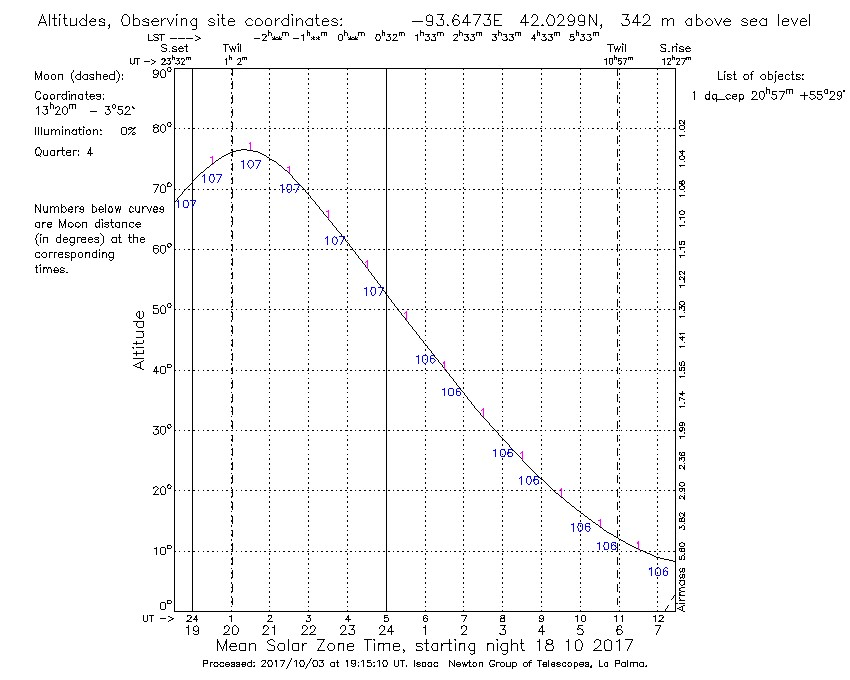
\includegraphics[width=\linewidth]{figs/staralt.png}
		\caption{Output from Peter Sorensen's Object Visibility applet. Peek is around 20:00:00 CST and is still sufficiently high four hours later at 24:00:00 CST}
		\label{fig:staralt}
	\end{figure}

\section{Scientific Justification}

\section{Technical Justification}

	Previous experiments done using the same telescope and SBIG CCD have shown that differential photometry can be accurate to around \SI{0.01}{mag}. Because our expected magnitude range is \SI{0.08}{mag} we wanted to be sure a difference could be seen. To showcase the precision we have already taken a preliminary dataset that shows a difference in the magnitudes. \autoref{fig:mags}

	\begin{figure}[p]
		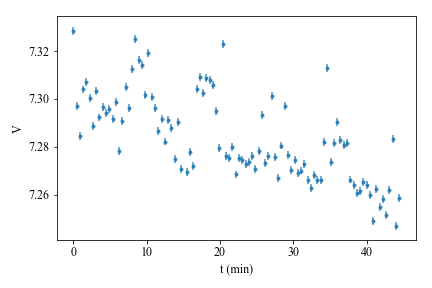
\includegraphics[width=\linewidth]{figs/mags.png}
		\caption{}
		\label{fig:mags}
	\end{figure}

\section{Analysis Plan}



%\bibliography{proposal}
%\bibliographystyle{plain}


\end{document}
